\section{方法设计}

本章给出本文方法的总体设计方案，并对各关键模块进行详细说明。

\subsection{总体设计方案}

【先用一段文字概括整体思路与技术路线，再给出总体框架图并对照图说明各部分的衔接关系。】

本文方法的总体框架如图 \ref{fig:overall} 所示，整体流程包括【阶段一】、【阶段二】与【阶段三】三个部分。首先，……；其次，……；最后，……。

\begin{figure}[htbp]
    \centering
    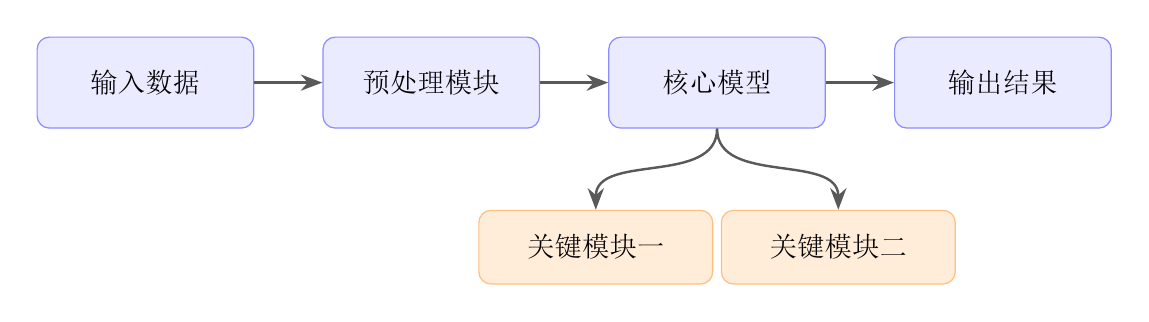
\includegraphics[width=0.9\textwidth]{images/overall_framework.png}
    \caption{总体框架图（示例，请替换为本人论文的框架图）}
    \label{fig:overall}
\end{figure}

\subsection{关键模块设计}

【分模块介绍设计细节，每个模块单独成段，必要时配合公式、伪代码或示意图说明。】

以【关键模块一】为例，其计算过程可以表示为：
\begin{equation}
  \mathbf{h} = \sigma\left(\mathbf{W}\mathbf{x} + \mathbf{b}\right)
\end{equation}
其中 \(\mathbf{W}\) 与 \(\mathbf{b}\) 为可学习参数，\(\sigma(\cdot)\) 为激活函数。

【关键模块二】的设计目标是……，具体实现上……。

\subsection{本章小结}

本章介绍了所提方法的总体设计与各关键模块的实现方式，下一章将通过实验对方法的有效性进行验证。
